% !TeX root = 2nd-course-in-latex.tex
\chapter{Presentations with Beamer}

If you ask me, Beamer is an odd tool.
Presentations are inherently visual,
so a programming tool like \LaTeX{} seems ill-suited for the job.
On the other hand, most graphical programs cannot match the quality of \LaTeX{} mathematics,
and technical talks often have modest visual needs.

Beamer does strike a nice balance between the two,
if only your talk is not too ambitious with the visuals.
At the same time I find its complexity to be similar to TikZ
-- a lot of things are possible, but not all of them are advisable.

\begin{practices}
Even though this course is not about presentation skills,
I want to use this opportunity for an important reminder:
Beamer makes it very easy to throw too much mathematics at your audience.

Leave whitespace on your slides, and focus on pictures to support your point.
If you want to dive deep into a mathematical topic,
there is an even superior tool: blackboard.
\end{practices}


%
%
\section{Basic structure}

Beamer is implemented as the \textbf{beamer} document class.
A minimal Beamer file is thus:
%
\begin{ExampleCode}
\documentclass{beamer}

\begin{document}

\begin{frame}
\end{frame}

\end{document}
\end{ExampleCode}
%
Beamer automatically loads \pkg[Beamer]{hyperref}.
It also loads \pkg[Beamer]{amsthm} and creates some theorem environments by default.

Since \TeX{} always believes it is typesetting for printing,
Beamer modifies the page size to be suitable.
By default it is $128 \times 96$~mm, which corresponds to 4:3 aspect ratio.

To modify the aspect ratio, you can pass the \verb|aspectratio| class option.
It is a string of two to four digits, and interpreted like:
\verb|aspectratio=32| means 3:2, \verb|169| means 16:9, and \verb|1610| means 16:10.

\begin{practices}
Many computer screens have 16:9 or 16:10 aspect ratio, so 4:3 might seem old-fashioned.
However, 4:3 has the benefit of increased vertical space.
Many projectors can output either aspect ratio comfortably.
If possible, check the venue beforehand.
\end{practices}

The default 11~pt font fits very nicely with the simulated paper size.
You can pass the \verb|10pt| or \verb|12pt| class options to modify the font size a bit.%
\footnote{There are also some more choices,
but they make the text either very large of very unreadable.}

\begin{gotcha}
You should put \verb|\usefonttheme{professionalfonts}| in the preamble
if you use \mbox{LuaTeX} or XeTeX.
It appears that Beamer does not always recognize that Latin Modern is in use with these compilers.
If the font theme is not changed,
Beamer might produce bad kerning for some specific letter combinations.
\end{gotcha}


For basic title design, you can use the usual \cmd{title}, \cmd{author}, and \cmd{date} commands.
There is also an \cmd{institute} command for specifying the author institution,
and a \cmd{titlegraphic} command that can be used for a logo etc.
Thus a basic presentation with just a title page is set with:
%
\begin{ExampleCode}
\title{My fantastic presentation}
\author{Firstname Lastname}
\institute{University of Puuhamaa}
\titlegraphic{\includegraphics[width=3cm]{TheDogs.jpg}}
\date{20 May 2024}

\begin{document}

\maketitle

\end{document}
\end{ExampleCode}
%
\EmbedPdfPage{examples/basic-beamer.pdf}{1}
%
(The \cmd{maketitle} command can be inside or outside a \verb|frame| environment.
The command is synonymous with \cmd{titlepage}.)

New slides are created with the \env{frame} environments.
Each slide acts like a page, so the basic typesetting commands are available.
The title for the frame can be set with \cmd{frametitle};
it is displayed in the frame header.
%
\begin{ExampleCode}
\begin{frame}
\frametitle{Hi there!}

Welcome to my presentation!

We will talk about Pythagoras and his theorem.
\end{frame}
\end{ExampleCode}
%
\EmbedPdfPage{examples/basic-beamer.pdf}{2}

Note that the paragraphs have no visual separation whatsoever.
You can of course set \cmd[Beamer]{parskip} to a better value
(I suggest a larger value than for printed documents, like 1~em),
but Beamer presentations are often composed of \emph{blocks}.
The \env{block} environment has a title and content:
%
\begin{ExampleCode}
\begin{frame}
\frametitle{Hi there!}

Welcome to my presentation!

\begin{block}{Goal}
You will learn about Pythagoras and his theorem.
\end{block}
\end{frame}
\end{ExampleCode}
%
\EmbedPdfPage{examples/basic-beamer.pdf}{3}
%
In this example the block is not very highlighted,
but that can be changed with a suitable colour theme.
We'll get to that in \Cref{sec:beamer styles}.

By default, Beamer creates a few common theorem environments.
More can be created with the usual \pkg[Beamer]{amsthm} commands (see \Cref{sec:amsthm}).
%
\begin{ExampleCode}
\begin{frame}
\frametitle{The theorem}

\begin{theorem}
If $a$ and $b$ are the lengths of catheti of a right-angled triangle,
then the hypothenuse has length $\sqrt{a^2 + b^2}$.
\end{theorem}
\begin{proof}
We'll get to this soon.
\end{proof}

\end{frame}
\end{ExampleCode}
%
\EmbedPdfPage{examples/basic-beamer.pdf}{4}


To highlight text, it is advisable to use the \cmd{alert} command.
By default it makes the text red, but the style can be customized.

The usual list environments can be used.
Beamer loads the \pkg{enumerate} package that enables a shorthand styling syntax
for \env[shorthand styles]{enumerate} environments.

Let us illustrate these elements with a multi-column layout.
Such a layout is created with a \env[Beamer]{columns} environment.
It takes an optional vertical alignment specifier (top by default;
vertical centres with \verb|c| and bottoms by \verb|b|).%
\footnote{If things do not align as you would expect,
you should also try the \texttt{T} option:
it aligns baselines of the first lines instead of tops of lines.}
%
Inside this environment, columns are created with the \env[Beamer]{column} environment,
which takes column width as a required argument.%
\footnote{There is also an equivalently named command
if you prefer to avoid deeply nested environments.}
%
\begin{ExampleCode}
\begin{columns}
\begin{column}{0.5\textwidth}

Properties of \alert{Pythagoras}:
\begin{enumerate}[1.]
    \item From Ancient Greece ...
\end{enumerate}
\end{column}

\begin{column}{0.5\textwidth}
Properties of \alert{the theorem}:
\begin{enumerate}[i)]
    \item Not invented by Pythagoras ...
\end{enumerate}

\end{column}
\end{columns}
\end{ExampleCode}
%
\EmbedPdfPage{examples/basic-beamer.pdf}{5}


\begin{gotcha}
Frames do not really support the \env[Beamer]{verbatim} environment;
the \pkg{listings} package is probably visually nicer anyways.
\end{gotcha}


%
%
\section{Including graphics}

The usual graphics commands of \LaTeX{} and TikZ can be used as usual.
Moreover, the usual \env[Beamer]{figure} and \env[Beamer]{table} environments can be used.
%
\begin{ExampleCode}
\begin{figure}
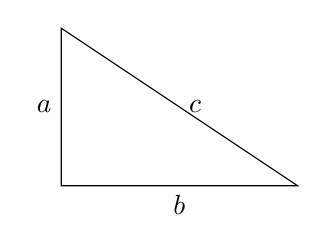
\begin{tikzpicture}
    \draw (0,0) -- (0,2) node[pos=0.5, left] {$a$}
        -- (3,0) node[pos=0.5, right] {$c$}
        -- cycle node[pos=0.5, below] {$b$};
\end{tikzpicture}
\caption{A right triangle.}
\end{figure}

\begin{figure}
    \includegraphics[width=3cm]{TheDogs.jpg}
\caption{Slide hijacked by a dog!}
\end{figure}
\end{ExampleCode}
%
\EmbedPdfPage{examples/basic-beamer.pdf}{6}

\begin{gotcha}
As with article classes, figures are not placed side by side.
The \pkg{subcaption} package is again useful for that;
see \Cref{sec:subfigures}.
Moreover, there is no automatic page breaking:
if you put too much stuff on a slide, they will overflow.
\end{gotcha}


If you need to position graphics absolutely,
you can use the absolute positioning system of TikZ (\Cref{sec:tikz absolute}).
For instance, the following code could be used as the basis of a slide header:
\begin{ExampleCode}
\begin{tikzpicture}[remember picture,overlay]
\node[yshift=0.15\paperheight] at (current page.center){%
\includegraphics[width=\paperwidth]{slideheader.jpg}};
\end{tikzpicture}
\end{ExampleCode}
This assumes the picture to be wide but narrow.
The code needs to be compiled twice before anything is visible.


\begin{warning}
You can find code examples and Beamer documentation about embedding video files inside a presentation.
This is a great way to make a presentation work only on a specific Acrobat Reader version
and only on your current computer.
It is 99~\% guaranteed not to work at a conference venue.

As annoying as it is to switch between programs to show videos,
it is the only reliable option.
\end{warning}

\begin{technote}
As with embedded videos, it is possible to specify slide transition effects,
but they might not work with all PDF viewers.
Because of this, we do not discuss them here.
\end{technote}



%
%
\section{Uncovering things}

The easiest way to uncover things piecewise is the \cmd{pause} command.
As the name suggests, it inserts a slide break at the source location.
%
\begin{ExampleCode}
\begin{frame}
\frametitle{A digression on numbers}

\begin{theorem}
Every natural number has a successor.
\end{theorem}

\pause

\begin{theorem}
There is at least one natural number.
\end{theorem}

\pause

\begin{corollary}
There are infinitely many natural numbers.
\end{corollary}
\end{frame}
\end{ExampleCode}
%
\begin{center}
\fbox{\includegraphics[page=7, width=0.3\textwidth]{examples/basic-beamer.pdf}}~
\fbox{\includegraphics[page=8, width=0.3\textwidth]{examples/basic-beamer.pdf}}~
\fbox{\includegraphics[page=9, width=0.3\textwidth]{examples/basic-beamer.pdf}}
\end{center}

The \cmd{pause} command can be used in many places:
between blocks and paragraphs and inside lists.

\begin{gotcha}
The \cmd{pause} command does not work inside \pkg[with Beamer]{amsmath} environments.
\future{Workarounds?}
\end{gotcha}

To get more control, it is possible to use the \cmd{uncover} command
and \emph{overlay specifications}.\index{overlay specification}
Here are some example overlay specifications:
\begin{description}
\item[\texttt{<2>}] Only shown on slide~2.
\item[\texttt{<2->}] Shown on slide~2 and all following slides.
\item[\texttt{<2-3,5>}] Shown on slides~2--3 and~5.
\end{description}
%
The block environments support overlay specifications,
so the previous example could be rewritten as:
%
\begin{ExampleCode}
\begin{frame}
\frametitle{A digression on numbers, version 2}

\begin{theorem}<1->
Every natural number has a successor.
\end{theorem}

\begin{theorem}<2->
There is at least one natural number.
\end{theorem}

\begin{corollary}<3->
There are infinitely many natural numbers.
\end{corollary}
\end{frame}
\end{ExampleCode}
%
There is also a shorthand syntax \verb|<+->| that is functionally similar to \cmd{pause}:
it increments the previous overlay specification by one.%
\footnote{To be precise, the magic command is \texttt{+}:
it is replaced by the previous slide number, and the slide number is then incremented.}
In the previous example, all overlay specifications could be replaced by \verb|<+->|.
This is particularly useful for lists:
%
\begin{ExampleCode}
\begin{itemize}
    \item<+-> This is shown starting from the first slide.
    \item<+-> This is shown starting from the second slide.
    \item<+-> This is shown starting from the third slide.
\end{itemize}
\end{ExampleCode}
%
Beamer introduces an optional argument to produce such lists with even less repetition:
%
\begin{ExampleCode}
\begin{itemize}[<+->]
    \item This is shown starting from the first slide.
    \item This is shown starting from the second slide.
    \item This is shown starting from the third slide.
\end{itemize}
\end{ExampleCode}

Outside an environment or list, the \cmd{uncover} command works the same:
%
\begin{ExampleCode}
\begin{frame}
\frametitle{On the infinitude of numbers}

\begin{corollary}
There are infinitely many natural numbers.
\end{corollary}
\begin{proof}
\uncover<2->{Suppose that $n$ is the largest natural number.}
\uncover<3->{But then its successor $n+1$ is an even larger natural number.}
\end{proof}

\end{frame}
\end{ExampleCode}
%
\begin{center}
\fbox{\includegraphics[page=10, width=0.3\textwidth]{examples/basic-beamer.pdf}}~
\fbox{\includegraphics[page=11, width=0.3\textwidth]{examples/basic-beamer.pdf}}~
\fbox{\includegraphics[page=12, width=0.3\textwidth]{examples/basic-beamer.pdf}}
\end{center}

Overlay specifications can also be applied to text styling commands like \cmd{alert}.
In this case, the text styling is only applied on the specified frames.
%
\begin{ExampleCode}
\begin{frame}

\textbf<1>{Bold on the first slide only.}\\
\alert<2>{Alerted on the second slide only.}

\end{frame}
\end{ExampleCode}
%
\begin{center}
\fbox{\includegraphics[page=13, width=0.45\textwidth]{examples/basic-beamer.pdf}}~
\fbox{\includegraphics[page=14, width=0.45\textwidth]{examples/basic-beamer.pdf}}
\end{center}

Lists have a special shorthand syntax for setting an element in alerted style.
An overlay specification like \verb|<alert@2>| will make the item alerted on the second slide only.
This can be combined with the \verb|+| syntax to simplify matters:
%
\begin{ExampleCode}
\begin{itemize} % Or put [<alert@+>] here
    \item<alert@+> This is highlighted on the first slide.
    \item<alert@+> This is highlighted on the second slide.
    \item<alert@+> This is highlighted on the third slide.
\end{itemize}
\end{ExampleCode}
%
If necessary, you can combine uncover and alert specifications with syntax like \verb+<1- | alert@2>+,
or the monstrous \verb&<+-|alert@+>& (which alerts on the same slide as where the item appears).

\begin{practices}
The Beamer manual advises against gradually revealing lists,
so making them all visible from the start,
but alerting each item in turn might be a better option.
\end{practices}


There is also an \cmd{only} command.
Its difference to the \cmd{uncover} command is that no space is reserved.
Since it may cause the positioning of the adjacent text change
between slides, it should only be used when necessary.
(This example also has some extra syntax described below.)
%
\begin{ExampleCode}
\begin{frame}<1-2>[label=surprise-dogs]

There is nothing to see here.\\
\only<2>{\includegraphics[width=6cm]{../pictures/TheDogs.jpg}\\}
Absolutely nothing at all.\\
\only<3>{\Large What was that?!}

\end{frame}
\end{ExampleCode}
%
\begin{center}
\fbox{\includegraphics[page=15, width=0.45\textwidth]{examples/basic-beamer.pdf}}~
\fbox{\includegraphics[page=16, width=0.45\textwidth]{examples/basic-beamer.pdf}}
\end{center}

It is possible to repeat a frame without duplicating the code.
In the previous example, we set a label for the frame.
The \cmd{againframe} command can be used to repeat a frame,
even if there were other frames in between.
This mechanism also works together with overlay specifications:
the above example only shows slides 1--2, and the next code shows the final slide:
%
\begin{ExampleCode}
\againframe<3>{surprise-dogs}
\end{ExampleCode}
%
\begin{center}
\fbox{\includegraphics[page=17, width=0.45\textwidth]{examples/basic-beamer.pdf}}
\end{center}


\begin{remark}
You can also uncover parts of a TiKZ picture gradually.
By default TikZ reserves space only for the visible elements;
to avoid elements moving around you can use the \cmd{useasboundingbox} command
we met on page~\pageref{ex:tikz useasboundingbox}.
\end{remark}


\future{reserving space for other elements}

%
%
%
\section{Sections and parts}

The \cmd[Beamer]{section} command can be used to organize your presentation into sections.
In some themes (see \Cref{sec:beamer styles}),
the current section -- and even progress within the section -- is displayed in the header.
As usual, a shorter section name can be passed in an optional argument.

The \cmd{sectionpage} command can be used to set a ``title page'' for the section.
(The default theme used in this example does not set it very beautifully.)
%
\begin{ExampleCode}
\section{Details of the proof}

\sectionpage
\end{ExampleCode}
%
\begin{center}
\fbox{\includegraphics[page=18, width=0.45\textwidth]{examples/basic-beamer.pdf}}
\end{center}

However, it might be more useful to create a frame that shows
the new section highlighted in the table of contents.
This can be achieved with
%
\begin{ExampleCode}
\begin{frame}
    \tableofcontents[currentsection]
\end{frame}
\end{ExampleCode}
%
Without the optional argument, an ordinary table of contents is printed.

It is possible to put ``backup'' slides in an appendix.
Any sections and frames following \cmd[Beamer]{appendix}
will not be shown in navigation bars in the header.

There are also similar subsection-level commands,
if you really need that level of granularity.
In the other end of the granularity spectrum,
the \cmd[Beamer]{part} command can also be used.
Each part is essentially its own isolated presentation
-- the table of contents only shows the current part, and so on.

You can create a bibliography with the manual method described in \Cref{sec:bibliography manual}.
The reason \emph{not} to use BibTeX is that the bibliography
might need to be broken across several frames.
(You can use the \verb|.bbl| file generated by BibTeX as a starting point, of course.)

\begin{practices}
Please think of your audience.
Throwing seventeen references at them in the last 20~seconds of your talk is beyond useless.
Consider using e.g.\ footnotes at the point of citation instead.
\end{practices}




%
%
%
\section{Styling it}\label{sec:beamer styles}

Like the rest of \LaTeX, Beamer attempts to separate content and presentation.
It does so via an extensive styling system.
The appearance of presentation is controlled with commands in the preamble.

First off, controlling the navigation symbols.
There are several styles for them, but I believe you only need one
-- the one where they are not shown:%
\footnote{Have you ever seen anyone use them?}
\begin{ExampleCode}
\beamertemplatenavigationsymbolsempty
\end{ExampleCode}

\begin{remark}
As mentioned above, if you use LuaLaTeX or XeLaTeX,
you should usually also specify
\begin{ExampleCode}
\usefonttheme{professionalfonts}
\end{ExampleCode}
to avoid small kerning issues with some characters.
\end{remark}


Some people prefer to show ``covered'' text in slightly transparent style,
so that the audience sees that it is there.
This can be controlled with the \cmd{setbeamercovered} command.
It takes one argument, and the common values for it are:
\begin{description}
\item[\texttt{invisible}] The default: covered text is invisible.
\item[\texttt{transparent}] Covered text is partially visible.
    This is in fact equivalent to \verb|transparent=15|, where the percentage can be tweaked.
\item[\texttt{dynamic}] The transparency effect depends on the number of slides until the piece is uncovered.
    Use with extreme caution, might be distracting.
\end{description}



%
%
\subsection{Themes}

Beamer comes with a complex theming system for changing the appearance of things.
Essentially, you should only need to modify the preamble to change how things look.

The overall appearance is determined by the \emph{presentation theme}.
It is chosen with \cmd{usetheme} in the preamble.
The presentation theme, in turn, consists of four parts, any of which can be changed independently:
\begin{description}
\item[Inner theme] The appearance of frame contents (blocks, lists, etc.)
    Changed with \cmd{useinnertheme}.
\item[Outer theme] The appearance of frame border (footer, navigation bar etc.)
    Changed with \cmd{useoutertheme}.
\item[Color theme] The colours used for elements.
    Individual colours can be further customized.
    Changed with \cmd{usecolortheme}.
\item[Font theme] The fonts to be used for elements.
    Also these can be customized individually.
    Changed with \cmd{usefonttheme}.
\end{description}
%
It is thus possible to start from a presentation theme,
and then change parts of the style to suit your artistic tastes.

The built-in presentation themes are showcased in \cite[Chapter~15]{beamer},
inner and outer themes in \cite[Chapter~16]{beamer},
and color and font themes in the following chapters.

In this example, we use the \verb|Madrid| presentation theme without any further customization:%
\footnote{Except for using \texttt{professionalfonts}, since the file was compiled with XeLaTeX.}
%
\begin{ExampleCode}
\title{My fantastic presentation}
\author[F.~Lastname]{Firstname Lastname}
\institute[U.~Puuhamaa]{University of Puuhamaa}
\date{20 May 2024}

\beamertemplatenavigationsymbolsempty
\usefonttheme{professionalfonts}
\usetheme{Madrid}
\end{ExampleCode}
%
\begin{center}
\fbox{\includegraphics[page=1, width=0.45\textwidth]{examples/beamer-theme.pdf}}~
\fbox{\includegraphics[page=2, width=0.45\textwidth]{examples/beamer-theme.pdf}}
\end{center}

Then, let us modify the look a bit.
We take the \verb|miniframes| outer theme into use;
it displays the sections and progress within section in the header.
We also use its optional argument to simplify the footer.
We then change to the \verb|crane| colour theme in order to induce a headache in our audience,
and use the default serif font:
%
\begin{ExampleCode}
\beamertemplatenavigationsymbolsempty
\usefonttheme{professionalfonts}
\usetheme{Madrid}
\useoutertheme[footline=authortitle]{miniframes}
\usecolortheme{crane}
\usefonttheme{serif}
\end{ExampleCode}
%
\begin{center}
\fbox{\includegraphics[page=1, width=0.45\textwidth]{examples/beamer-theme2.pdf}}~
\fbox{\includegraphics[page=2, width=0.45\textwidth]{examples/beamer-theme2.pdf}}
\end{center}



%
%
\subsection{Colours}

\begin{practices}
It is \emph{extra important} to take care of colour contrast in presentations.
Projectors have a far smaller colour range than computer displays,
especially if the room is bright.
What might appear like two distinct colours on your laptop
might be indistinguishable when projected.
\end{practices}

If the colour scheme provided by \cmd{usecolortheme} is still not what you want,
it is possible to tweak the individual colours.
This is done with \cmd{setbeamercolor}.

Beamer uses named colours for everything.
For example, the \verb|block body| colour is used inside all \env{block} environments.
Each colour also has two components: foreground (\verb|fg|) and background (\verb|bg|).
These can be set to any values supported by \pkg{xcolor}.

For example, here we change the foreground colour of block titles,
and both the foreground and background colours of block bodies:%
\begin{ExampleCode}
\setbeamercolor{block title}{fg=red}
\setbeamercolor{block body}{fg=white, bg=blue}
\end{ExampleCode}
%
\begin{center}
\fbox{\includegraphics[page=3, width=0.6\textwidth]{examples/beamer-theme2.pdf}}
\end{center}

Some of these colours are also inherited from ``parent colours''.
Maybe the most interesting of these is \verb|structure|,
which applies to all frame and block headings, unless overridden by a child style.
The colour of the ``background canvas'' is determined by the \verb|bg| colour of \verb|normal text|.

You can find the full list of predefined colours in the Beamer documentation for each element type.
The source code of each Beamer colour theme is also very readable,
and can be used as a reference.%
\footnote{Where your particular \LaTeX{} installation puts package sources might be complicated.
For Beamer, the source is also available on Github:
\url{github.com/josephwright/beamer}.}



\subsection{Fonts}

\begin{practices}
Beamer uses a sans-serif font by default.
This is a good choice since sans-serif fonts are usually more readable in low resolution.
However, a serif font can be used to give a nice classic look.

Using \emph{italic} for emphasis might be too subtle;
prefer alerted and boldface text in presentations.
\end{practices}

As with colours, Beamer comes with a few built-in font themes
accessible with \cmd{usefonttheme}.
In addition to the \verb|professionalfonts| mentioned above
(which just disables some internal features, and can be used together with another font theme),
there is the sans-serif \verb|default|, its counterpart \verb|serif|,
and a few others that modify headings only \cite[Section~18.1]{beamer}.

The font size is controlled with the package options.
Moreover, since Beamer uses the default serif and sans-serif fonts,
you can replace the fonts with the methods described in \Cref{sec:typefaces}.

If you really need to customize the font used for a particular element,
there is a system similar to the one used for colours.
The \cmd{setbeamerfont} command takes the element name and a list of attributes to override.
The attributes are \verb|size|, \verb|shape|, \verb|series|, and \verb|family|,
and their possible values are the declarations listed in \Cref{sec:font attributes}.

In this (now awfully ugly) example,
we modify the frame title to be in bold, sans-serif font:
\begin{ExampleCode}
\setbeamerfont{frametitle}{series=\bfseries, family=\sffamily}
\end{ExampleCode}
%
\begin{center}
\fbox{\includegraphics[page=4, width=0.6\textwidth]{examples/beamer-theme2.pdf}}
\end{center}



%
%
\subsection{Templates}

Finally, the appearance of repeated elements like titles can be controlled by \emph{templates}.
Since this goes deeper into the internals of Beamer,
we only refer to the documentation \cite[Section~16.3]{beamer}.


%
%
\section{Handouts}

To produce handouts, pass the \verb|handout| optional argument to the document class.
In this mode, the overlays are ``flattened'' so that everything is visible at once.

If you still need to split a frame into multiple parts in the handout,
you can modify the overlay specification to also apply to handouts.\index{overlay specification!handout}
The following code shows its contents on the third slide in presentation mode,
and on the second slide in handout mode:
\begin{ExampleCode}
\only<3|handout:2>{...}
\end{ExampleCode}

To suppress the inclusion of a frame,
you can put \verb|<handout:0>| immediately after \verb|\begin{frame}|.
This overlay specification means that only the 0th slide of the frame will be printed in the handout
-- which does nothing, since the slide numbers start at 1.

